\chapter{\IfLanguageName{dutch}{Uitwerking}{Results}}%
\label{ch:uitwerking}

\section{Keuze van technologieën}

In de literatuurstudie en probleemanalyse zijn verschillende technologieën en API's onderzocht die kunnen worden gebruikt voor het genereren van looproutes en het opvragen van weersverwachtingen. Deze keuze is gebaseerd op de behoeften en vereisten van het project, evenals op de technische vaardigheden en voorkeuren van de ontwikkelaar.

\vspace{1cm}

Als API's zijn de volgende geselecteerd:
\begin{itemize}
    \item \textbf{OpenWeatherMap API} voor het opvragen van weersverwachtingen
    \item \textbf{Overpass API/OpenStreetMap} voor het genereren van tussenpunten op een route
    \item \textbf{Google Maps API} voor het genereren en visualiseren van de looproutes.
\end{itemize}

\vspace{1cm}

Voor de ontwikkeling van de mobiele applicatie is gekozen voor het React Native framework, dat het mogelijk maakt om cross-platform applicaties te ontwikkelen met behulp van JavaScript en React. Dit biedt de mogelijkheid om zowel een iOS- als een Android-applicatie te ontwikkelen met een enkele codebase, wat de ontwikkelingstijd en -kosten aanzienlijk kan verminderen. De applicatie zal worden ontwikkeld en getest op een Windows-computer met behulp van de Android Studio-emulator. iOS-ondersteuning zal niet worden getest vanwege de beperkte tijd en middelen die beschikbaar zijn voor het project.

\vspace{1cm}


Voor de backend van de applicatie is gekozen voor Node.js, een JavaScript runtime die het mogelijk maakt om server-side applicaties te ontwikkelen met behulp van JavaScript. Dit biedt de mogelijkheid om een RESTful API te ontwikkelen voor het opvragen van weersverwachtingen en het genereren van looproutes. Meer specifiek zal Express.js worden gebruikt als webframework voor het ontwikkelen van de API.

\vspace{1cm}


Voor zowel frontend als backend wordt Typescript gebruikt. Typescript is een superset van JavaScript die het mogelijk maakt om statische types toe te voegen aan JavaScript-code. Dit biedt de mogelijkheid om fouten op te sporen en de codebase te structureren en te documenteren.

\vspace{1cm}


Voor de database van de applicatie is er besloten om enkel offline data op te slaan. Dit gebeurt via AsyncStorage van react-native-asyncstorage. Dit maakt het mogelijk om key-values op te slaan. 
Er is besloten om geen online database in de backend te voorzien. Dit komt voornamelijk door een tijdsgebrek.
Er kan nog steeds een wordt een MySQL database gebruikt, die het mogelijk maakt om gegevens op te slaan en te beheren in een relationele database. Dit biedt de mogelijkheid om gebruikersgegevens en route-informatie op te slaan en te beheren in een gestructureerde en schaalbare database.

\vspace{1cm}


Verder wordt er voor authenticatie en autorisatie gebruik gemaakt van Auth0, een Identity-as-a-Service (IDaaS) platform dat het mogelijk maakt om gebruikers te authenticeren en autoriseren met behulp van verschillende methoden, zoals e-mail en wachtwoord, sociale logins en multi-factor authenticatie. Voor dit project zal er enkel gebruik gemaakt worden van e-mail en wachtwoord authenticatie.

\section{Architectuur}

De architectuur van de applicatie bestaat uit een frontend en een backend, die met elkaar communiceren via een RESTful API. De frontend is een mobiele applicatie die is ontwikkeld met behulp van het React Native framework, terwijl de backend een Node.js server is die is ontwikkeld met behulp van Express.js.

\vspace{1cm}


De frontend van de applicatie gebruikt Auth0 voor authenticatie en autorisatie, en communiceert met de backend via HTTP-requests. Er wordt een offline-first benadering gevolgd, waarbij gegevens worden opgeslagen in de lokale opslag van de mobiele applicatie.

\vspace{1cm}


De backend van de applicatie krijgt gegevens binnen van de frontend en communiceert verder met de Overpass API, Google Maps API en OpenWeatherMap API. De backend is afgeschermd met Auth0, zodat alleen geauthenticeerde gebruikers toegang hebben tot de API. Dit is echter uitgeschakeld voor het genereren van routes door problemen met het valideren van de token vanuit de mobiele applicatie.

\vspace{1cm}


De architectuur van de applicatie is ontworpen met het oog op schaalbaarheid, onderhoudbaarheid en uitbreidbaarheid zodat deze kan worden uitgebreid en aangepast naarmate de behoeften van de gebruiker veranderen. Verdere details over de architectuur van de applicatie zullen worden beschreven in de volgende hoofdstukken.

\section{Ontwerp}

Nu volgt de fase van ontwerp, waarbij de architectuur en functionaliteiten van de applicatie worden bepaald. Het doel van deze fase is om een duidelijk beeld te krijgen van hoe de applicatie eruit zal zien en welke functionaliteiten deze zal bevatten. Dit wordt bereikt door het maken van wireframes en mock-ups van de gebruikersinterface en het definiëren van de interacties en workflows van de applicatie.

\vspace{1cm}


Het ontwerp van de applicatie is gebaseerd op de gewenste features die zijn geïdentificeerd in de literatuurstudie en probleemanalyse. Hierbij wordt rekening gehouden met de behoeften en voorkeuren van de doelgroep, evenals met de technische mogelijkheden van de geselecteerde API's. Het doel is om een intuïtieve en gebruiksvriendelijke applicatie te ontwerpen die voldoet aan de verwachtingen van de gebruiker en aansluit bij de huidige trends in de markt voor routeplanning-apps.

\vspace{1cm}


Het ontwerp van de applicatie zal niet exact overeenkomen met de uiteindelijke applicatie, maar dient als leidraad voor de ontwikkeling ervan. Door het ontwerp te visualiseren in wireframes en mock-ups, kan de functionaliteit en gebruikerservaring van de applicatie worden gevalideerd. Vanwege tijdsbeperkingen en de complexiteit van de applicatie zal voornamelijk de functionaliteit worden gevolgd in plaats van de stijl van het ontwerp.

\subsection{Functionaliteiten en Flow van de applicatie}

De applicatie bestaat uit verschillende schermen en functionaliteiten die de gebruiker in staat stellen om een looproute te genereren. Concreet bestaan er 6 schermen in de applicatie:

\vspace{1cm}


\begin{itemize}
    \item \textbf{Home Scherm}: Hier kan de gebruiker een looproute genereren op basis van zijn huidige locatie en weersverwachting.
    \item \textbf{Route Scherm}: Hier kan de gebruiker de details van de gegenereerde looproute bekijken en opslaan voor later gebruik.
    \item \textbf{Settings Scherm}: Hier kan de gebruiker de instellingen van de applicatie aanpassen.
    \item \textbf{Overzicht Routes Scherm}: Hier kan de gebruiker de opgeslagen looproutes bekijken en beheren.
    \item \textbf{Route Creatie Scherm}: Hier kan de gebruiker een looproute genereren op basis van specifieke parameters.
    \item \textbf{Route Details Scherm}: Hier kan de gebruiker de details van een specifieke looproute bekijken en bewerken.
\end{itemize}

\vspace{1cm}


De flow van de applicatie begint bij het inloggen op de applicatie, waarna de gebruiker wordt doorgestuurd naar het Home Scherm. In de Proof of Concept zal dit scherm niet volledig worden geïmplementeerd, in de toekomst is het mogelijk om hier data van de gebruiker te tonen. Dan wordt via een drawer menu genavigeerd naar de verschillende schermen van de applicatie. De mogelijke navigaties zijn hier het Saved Routes Scherm en Settings Scherm. Op het Settings Scherm kan de gebruiker de instellingen van de applicatie aanpassen, zoals de eenheid van de afstand. Op het Saved Routes Scherm staat een overzicht van alle routes die zijn opgeslagen door de gebruiker, er is een onderscheid tussen routes die worden gegenereerd op basis van afstand of tijd. Hier kan de gebruiker een route selecteren om de details te bekijken. Verder is er een plus knop die de gebruiker naar het Route Create Scherm brengt, waar de gebruiker een route kan genereren op basis van specifieke parameters. Eens alle parameters zijn ingevuld, kan de gebruiker de route genereren en wordt deze doorgestuurd naar het Route Scherm. Hier kan een gebruiker een weerbericht opvragen voor de route. De gebruiker kan de route opslaan om later te lopen of meteen starten.

\subsection{Mock-ups}

De mock-ups van de applicatie zijn gemaakt met behulp van moqups, een online tool voor het maken van wireframes en mock-ups. De mock-ups zijn bedoeld als visuele representatie van het ontwerp van de applicatie en dienen als leidraad voor de ontwikkeling ervan.

    \begin{figure}[H]
        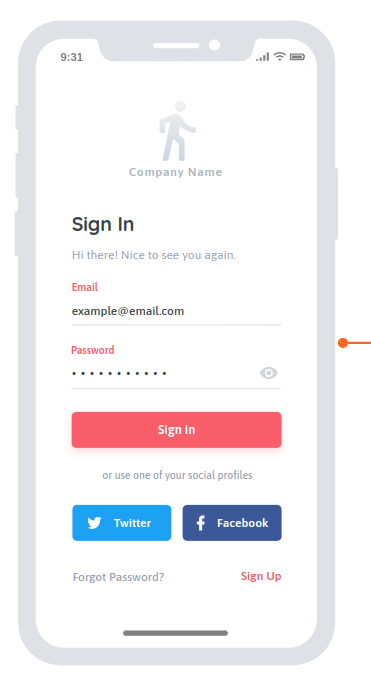
\includegraphics[width=20em]{./graphics/login_Mockup.png}
        \centering
        \caption{Mock up Login}
        \label{fig:loginMockup}
    \end{figure}

    \begin{figure}[H]
        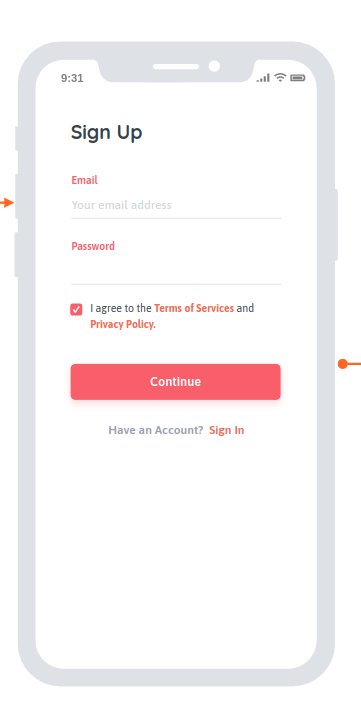
\includegraphics[width=20em]{./graphics/register_Mockup.png}
        \centering
        \caption{Mock up Register}
        \label{fig:registerMockup}
    \end{figure}
    
    \begin{figure}[H]
        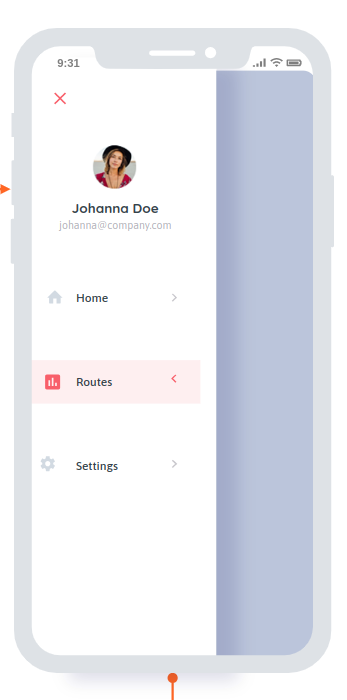
\includegraphics[width=20em]{./graphics/drawer_Mockup.png}
        \centering
        \caption{Mock up Drawer menu}
        \label{fig:DrawerMockup}
    \end{figure}

    \begin{figure}[H]
        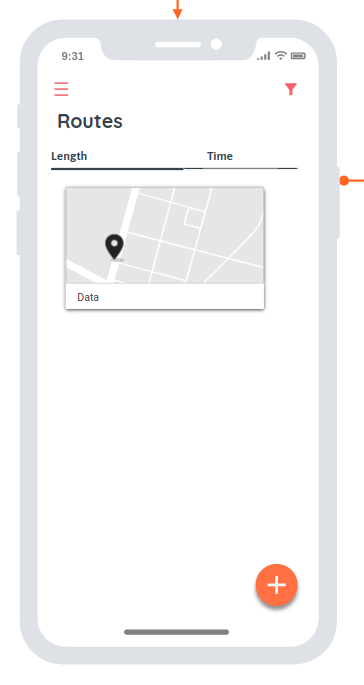
\includegraphics[width=20em]{./graphics/routeView_Mockup.png}
        \centering
        \caption{Mock up Route View}
        \label{fig:routeViewMockup}
    \end{figure}

    \begin{figure}[H]
        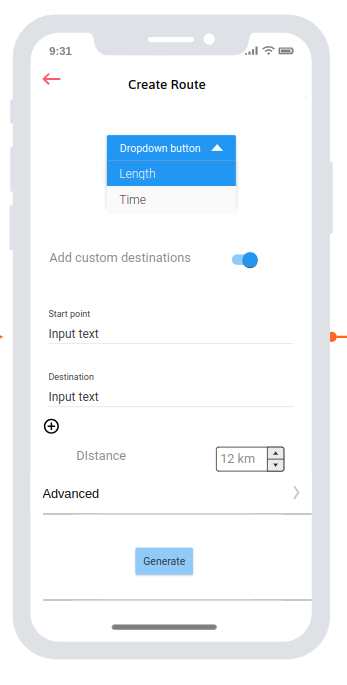
\includegraphics[width=20em]{./graphics/createRoute_Mockup.png}
        \centering
        \caption{Mock up Route Create}
        \label{fig:createRouteMockup}
    \end{figure}

    \begin{figure}[H]
        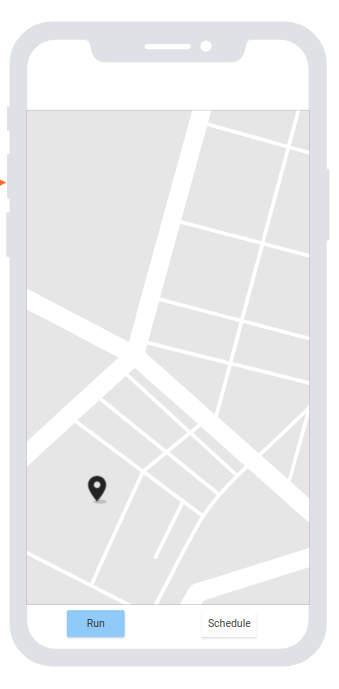
\includegraphics[width=20em]{./graphics/route_Mockup.png}
        \centering
        \caption{Mock up Route}
        \label{fig:routeMockup}
    \end{figure}

    \pagebreak

    \section{Proof of Concept}

    Na het ontwerp volgt de fase van ontwikkeling en implementatie. Hier wordt een Proof of Concept ontwikkeld, 
    bestaande uit zowel een online backend als een mobiele applicatie.

    \vspace{1cm}


    De code is beschikbaar op Github. 

    \vspace{1cm}

    De frontend \url{https://github.com/LaurensDM/RunnerApp}.
    
    \vspace{1cm}

    De backend \url{https://github.com/LaurensDM/RunnerApp-API}

    \subsection{Frontend}

    react-native-paper en react-native-navigation worden gebruikt voor styling en navigatie. 
    De applicatie is opgedeeld in verschillende componenten, 
    zoals HomeScherm, RouteScherm, SettingsScherm, SavedRoutesScherm, RouteCreateScherm en RouteDetailsScherm. 
    De navigatie tussen de verschillende schermen gebeurt via een drawer menu. 
    De applicatie maakt gebruik van Auth0 voor authenticatie en autorisatie. 
    De gebruiker kan inloggen met zijn e-mail en wachtwoord en wordt doorgestuurd naar het HomeScherm. 
    Gegevens worden opgeslagen in de lokale opslag van de mobiele applicatie via AsyncStorage.

    \vspace{1cm}


    Om een route te genereren is een internetverbinding nodig, 
    maar een gebruiker kan een bestaande route terug ophalen en bekijken zonder internetverbinding. Deze exacte route kan dan opnieuw gelopen worden. Aanpassingen aan de route kunnen enkel gebeuren met een internetverbinding.

    \vspace{1cm}

    
    Hier is een overzicht van de verschillende schermen van de applicatie:

    \vspace{1cm}

    
    Eerst wordt de gebruiker gevraagd om in te loggen. Hierbij wordt de gebruiker doorverwezen naar een browser waar Auth0 de authenticatie regelt.

    \begin{figure}[htbp]
        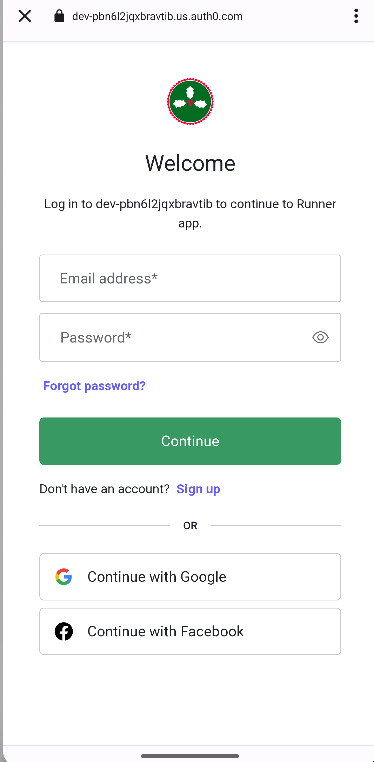
\includegraphics[width=20em]{./graphics/login.png}
        \centering
        \caption{Login}
        \label{fig:login}
    \end{figure}

    Vervolgens komt de gebruiker op het Home Scherm terecht. Voor de Proof of Concept staat hiet niet veel, 
    maar in de toekomst kan hier data van de gebruiker getoond worden.

    \begin{figure}[H]
        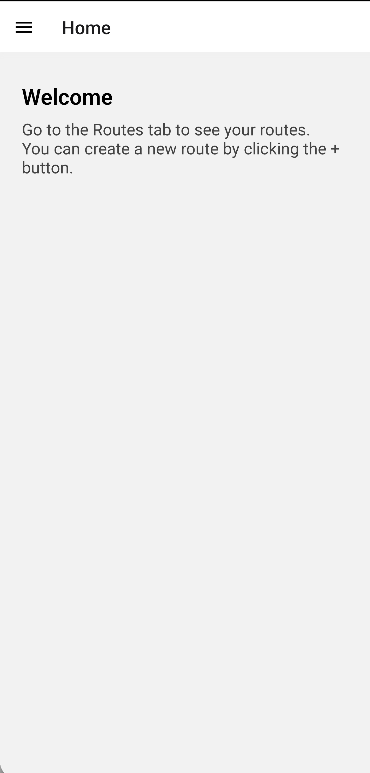
\includegraphics[width=20em]{./graphics/home.png}
        \centering
        \caption{Home}
        \label{fig:home}
    \end{figure}

    Via het drawer menu kan de gebruiker navigeren naar de verschillende schermen van de applicatie.

    \begin{figure}[H]
        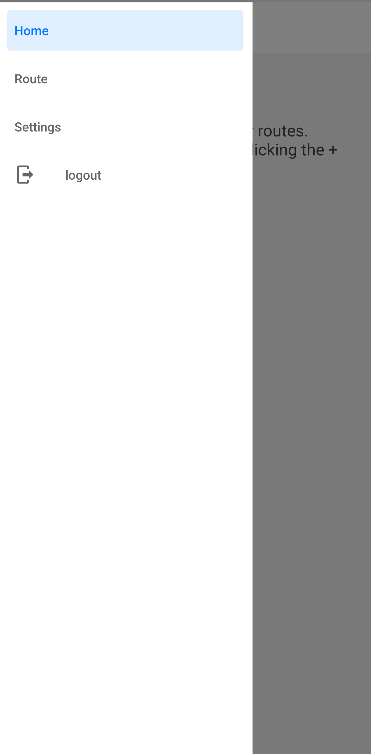
\includegraphics[width=20em]{./graphics/drawer.png}
        \centering
        \caption{Drawer}
        \label{fig:drawer}
    \end{figure}

    Op het Route Overzicht scherm kan de gebruiker de opgeslagen routes bekijken en beheren. Het is mogelijk op een route te selecteren om de details te bekijken. Hierbij wordt de route opgehaald uit de lokale opslag van de mobiele applicatie. Het is hier mogelijk om een nieuwe route te genereren met dezelfde parameters als de geselecteerde route, of om de route gewoon opnieuw te lopen.

    \vspace{1cm}


    Er is een onderscheid tussen routes gebaseerd op afstand en tijd. Er is geen verschil in de route die wordt gegenereerd. Bij een route op tijd wordt de afstand berekent op basis van de loopsnelheid van de gebruiker. Deze kan ingesteld worden in de Settings van de applicatie.

    \begin{figure}[H]
        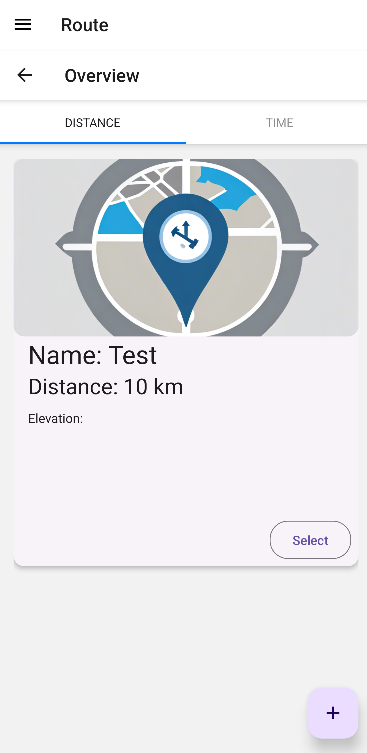
\includegraphics[width=20em]{./graphics/routes.png}
        \centering
        \caption{Routes}
        \label{fig:routes}
    \end{figure}

    Er is een plus knop die de gebruiker naar het Route Creatie scherm brengt. Hier kan de gebruiker een route genereren op basis van specifieke parameters. Eens alle parameters zijn ingevuld, kan de gebruiker de route genereren en wordt deze doorgestuurd naar het Route scherm.

    \begin{figure}[H]
        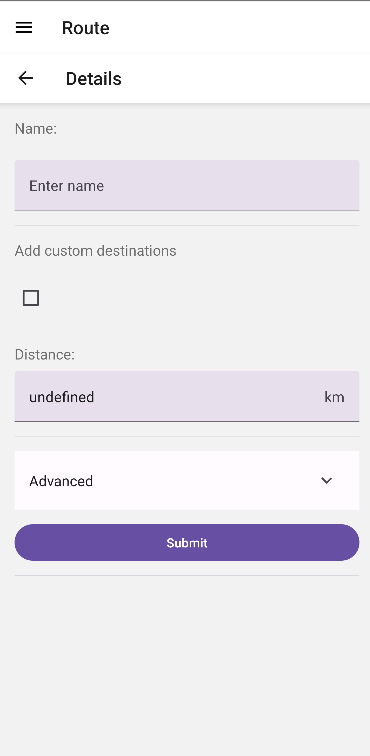
\includegraphics[width=20em]{./graphics/create.png}
        \centering
        \caption{Create Route}
        \label{fig:createRoute}
    \end{figure}

    Op het Route scherm kan de gebruiker de details van de gegenereerde route bekijken. Hier kan de gebruiker ook een weerbericht opvragen voor de route. De gebruiker kan de route opslaan om later te lopen of meteen starten.

    \begin{figure}[H]
        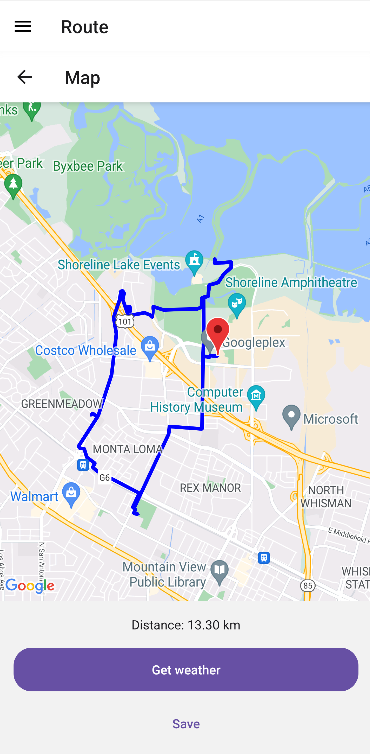
\includegraphics[width=20em]{./graphics/route.png}
        \centering
        \caption{Route}
        \label{fig:route}
    \end{figure}

    \begin{figure}[H]
        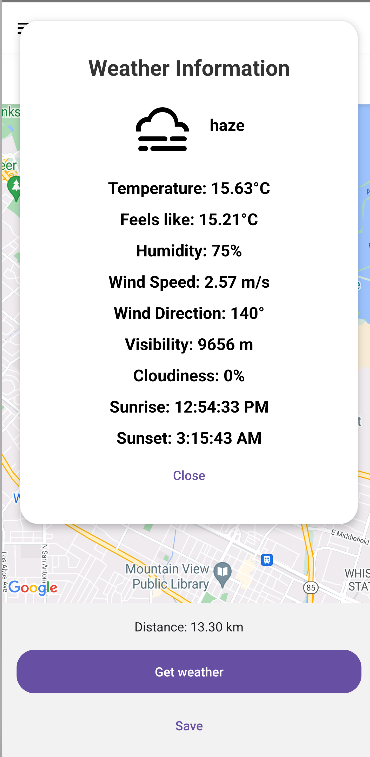
\includegraphics[width=20em]{./graphics/weather.png}
        \centering
        \caption{Weer}
        \label{fig:weather}
    \end{figure}

    Er is ook een instellingen scherm waar de gebruiker de instellingen van de applicatie kan aanpassen, zoals de loopsnelheid.

    \begin{figure}[H]
        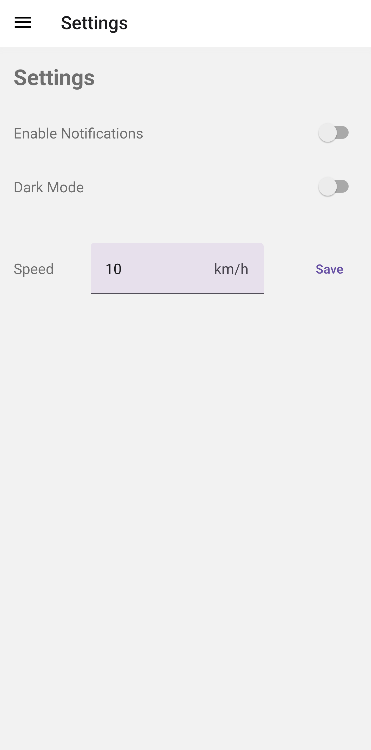
\includegraphics[width=20em]{./graphics/settings.png}
        \centering
        \caption{Instellingen}
        \label{fig:settings}
    \end{figure}


    \subsection{Backend}
    
    De backend is ontwikkeld met behulp van Node.js en Express.js en communiceert met de frontend via een RESTful API. 
    Auth0 wordt gebruikt voor authenticatie en autorisatie.
    De backend communiceert verder met de Overpass API, Google Maps API en OpenWeatherMap API voor het genereren van looproutes en het opvragen van weersverwachtingen.

    \vspace{1cm}

    
    Hier is een overzicht van de verschillende endpoints van de API. Er zijn andere endpoints ingesteld, maar de enigen die momenteel werken zijn de endpoints voor het genereren van een route en het ophalen van een weersvoorspelling.
    \begin{itemize}
        \item POST /api/route/
        \item POST /api/weather/
    \end{itemize}
  
    \vspace{1cm}


    Deze zijn de andere endpoints die ingesteld zijn, maar niet werken.
    \begin{itemize}
        \item POST /api/
        \item GET /api/user/
        \item GET /api/route/
        \item PUT /api/route/:id
        \item DELETE /api/route/:id
    \end{itemize}

    \vspace{1cm}

    
    Het genereren van een route gebeurt in verschillende stappen. 
    De API krijgt eerst de nodige data binnen van de frontend, zoals de locatie van de gebruiker, de gewenste afstand of tijd van de route en verdere geavanceerde opties. 
    De API valideert eerst of alle nodige parameters aanwezig zijn met behulp van express-validator. 

    \vspace{1cm}

    Vervolgens wordt een functie aangeroepen die de Overpass API aanspreekt om tussenpunten te genereren op basis van de gegeven parameters. 
    Functies die de Overpass API en Google Maps API aanspreken zijn gedefinieerd in een helpers folder, zodat er makkelijk integraties met andere platformen kunnen worden toegevoegd. 

    \vspace{1cm}

    Met de tussenpunten wordt een for-loop gestart die de afstand tussen de tussenpunten berekent. Ook wordt hier de hoogte van de verschillende tussenpunten berekent en worden tussenpunten gefilterd 
    op basis van de gewenste hoogte die de gebruiker heeft gespecifieerd. Dit gebeurt aan de hand van de Google Maps API.
    Als de afstand tussen de tussenpunten groter is dan de gewenste afstand van de route,
    wordt de loop beëindigd zonder dat alle tussenpunten zijn inbegrepen. 

    \vspace{1cm}

    In het geval dat er geen tussenpunten zijn teruggevonden, wordt een tussenpunt gegenereerd op basis van de locatie van de gebruiker, die zich dan op een aantal kilometers van de startlocatie bevindt. 
    De route wordt teruggegeven aan de frontend.

    \pagebreak

Dit is de code die verantwoordelijk is voor het genereren van de route.

\begin{lstlisting}
    async function generateRunningRoute({ startPoint, endPoint, waypoints, distance, advancedOptions }: RouteProps) {

    const generatedWaypoints = await getGeneratedWaypoints(distance!, startPoint, advancedOptions.poiTypes, advancedOptions.surfaceType);


    const runningRouteWaypoints: Waypoint[] = [];

    generatedWaypoints.sort((a, b) => {
        return calculateDistance(startPoint, a) - calculateDistance(startPoint, b);
    });

    let accumulatedDistance = 0;


    const elevationWaypoints = await calculateElevation([startPoint, ...generatedWaypoints.slice(0, 510), endPoint]);

    const filteredWaypoints = elevationWaypoints.filter((waypoint) => {
        const elevationChange = Math.abs(waypoint.elevation - elevationWaypoints[0].elevation); // Assuming startPoint elevation as reference
        if (elevationChange < 50) { // Adjust thresholds for flat, medium, and steep as needed
            return advancedOptions.height === 'flat';
        } else if (elevationChange < 100) {
            return advancedOptions.height === 'medium';
        } else {
            return advancedOptions.height === 'steep';
        }
    });

    const accumulatedWaypoints = filteredWaypoints != undefined && filteredWaypoints.length > 2 ? filteredWaypoints : generatedWaypoints;
    const allWaypoints = [...waypoints.sort((a, b) => calculateDistance(startPoint, a) - calculateDistance(startPoint, b)), ...accumulatedWaypoints];
    
    console.log('All waypoints:', allWaypoints.length);
    console.log(allWaypoints);
    
    const waypointLimit = 25;
    let timeOut = 0;
    if (allWaypoints.length === 0) {
        let currentPoint = startPoint;
        while (accumulatedDistance < distance * 1000) { // Convert km to meters
            // Find the next point along the route
            const nextPoint = findNextPoint(currentPoint, endPoint, distance * 1000 - accumulatedDistance, (distance / 6 * 1000));
            const calculatedDistance = calculateDistance(currentPoint, nextPoint);

            // Add the next point to the running route waypoints
            runningRouteWaypoints.push(nextPoint);
            accumulatedDistance += calculatedDistance;

            // Update currentPoint for the next iteration
            console.log(currentPoint);

            currentPoint = nextPoint;
            if (timeOut > 1000 || runningRouteWaypoints.length === 4) {
                break;
            }
            timeOut++;
        }
    } else {
        for (let i = 0; i < allWaypoints.length; i++) {
            const previousWaypoint = i === 0 ? startPoint : allWaypoints[i - 1];
            const waypoint1 = allWaypoints[i];
            const calculatedDistance = calculateDistance(previousWaypoint, waypoint1);
            const distanceToEnd = calculateDistance(waypoint1, endPoint);
            // accumulatedDistance += (accumulatedDistance + calculatedDistance) > distance *1000 ? 0 : calculatedDistance;
            if ((accumulatedDistance + calculatedDistance) > distance * 1000 || accumulatedDistance + distanceToEnd > distance * 1000) {
                accumulatedDistance += 0;
            } else {
                accumulatedDistance += calculatedDistance;
            }

            if (accumulatedDistance <= distance * 1000) { // Convert km to meters
                runningRouteWaypoints.push(waypoint1);
            } else {
                console.log(accumulatedDistance);
                break;
            }

            //Only 25 waypoints are allowed in a single request
            if (runningRouteWaypoints.length === waypointLimit) {
                console.log(accumulatedDistance);
                break;
            }
        }
    }
    runningRouteWaypoints.sort((a, b) => {
        return calculateDistance(a, endPoint) - calculateDistance(b, endPoint);
    });

    console.log('Running route waypoints:', runningRouteWaypoints.length);

    console.log(runningRouteWaypoints);



    // Generate route using Google Maps Directions API
    try {
        const createdRoute = await generateGoogleRoute(startPoint, endPoint, runningRouteWaypoints);
        return createdRoute.routes;
    } catch (error: any) {
        console.error('Error fetching route:', error.response.data);
        return null;
    }
}
\end{lstlisting}

Deze functie genereert een hardlooproute op basis van een aantal parameters. Waaronder een startpunt, een eindpunt, tussenpunten, de afstand van de route en geavanceerde opties.

\vspace{1cm}

De functie begint met het ophalen van gegenereerde tussenpunten met behulp van de getGeneratedWaypoints functie. Deze functie roept de Overpass API aan en genereert tussenpunten op basis van de gegeven parameters.
Er worden maximum 50 tussenpunten gegenereerd per parameter.
Deze gegenereerde tussenpunten worden vervolgens gesorteerd op basis van hun afstand tot het startpunt. De afstand wordt berekend met behulp van de calculateDistance functie.

\vspace{1cm}

Vervolgens wordt de hoogte van de route berekend met behulp van de calculateElevation functie. Deze functie roept de Google Maps Elevation API aan en berekent de hoogte van de verschillende tussenpunten. 
Hieraan worden enkel 510 tussenpunten meegegeven, omdat de Google Maps Elevation API een limiet heeft van 512 punten per aanvraag.
Er wordt gekeken naar het hoogteverschil tussen de verschillende tussenpunten en op basis daarvan worden de tussenpunten gefilterd. Dit wordt gedaan op basis van de geavanceerde opties die zijn meegegeven.

\vspace{1cm}

De gefilterde tussenpunten worden toegevoegd aan de lijst met alle tussenpunten. Als er geen tussenpunten zijn gegenereerd, worden er nieuwe tussenpunten gecreëerd door middel van de findNextPoint functie. 
Deze functie zoekt naar het volgende punt langs de route en voegt dit toe aan de lijst met tussenpunten. In totaal worden 4 tussenpunten gegenereerd die verspreid zijn in een radius die gelijk is aan de afstand van de route.
Dit wordt herhaald totdat de totale afstand van de route overeenkomt met de gewenste afstand of tot er 4 tussenpunten berekent zijn.

\vspace{1cm}

Als er wel tussenpunten zijn, dan worden deze toegevoegd aan de lijst met tussenpunten. Er wordt gekeken naar de afstand tussen de tussenpunten en of deze afstand past binnen de gewenste afstand van de route. 
Als de afstand tussen twee tussenpunten te groot is, wordt deze tussenpunt niet toegevoegd aan de lijst.

\vspace{1cm}

Er mag maximaal gebruik worden gemaakt van 25 tussenpunten in een enkele aanvraag. Als er meer tussenpunten zijn dan dit, dan worden alleen de eerste 25 tussenpunten gebruikt.
Dit is de limiet van de Google Maps Directions API.

\vspace{1cm}

Als de lijst met tussenpunten compleet is, dan wordt er met behulp van de Google Maps Directions API een route gegenereerd. 
Deze route wordt teruggegeven als resultaat van de functie. Als er een fout optreedt bij het ophalen van de route, dan wordt er null teruggegeven.